\documentclass{standalone}
\usepackage{graphicx}	
\usepackage{amssymb, amsmath, amsthm}
\usepackage{color}

\usepackage{tikz}
\usetikzlibrary{intersections, backgrounds, math}

\definecolor{light}{RGB}{220, 188, 188}
\definecolor{mid}{RGB}{185, 124, 124}
\definecolor{dark}{RGB}{143, 39, 39}
\definecolor{highlight}{RGB}{180, 31, 180}
\definecolor{darkteal}{RGB}{29, 79, 79}
\definecolor{darkolive}{RGB}{97, 123, 45}
\definecolor{gray10}{gray}{0.1}
\definecolor{gray20}{gray}{0.2}
\definecolor{gray30}{gray}{0.3}
\definecolor{gray40}{gray}{0.4}
\definecolor{gray60}{gray}{0.6}
\definecolor{gray70}{gray}{0.7}
\definecolor{gray80}{gray}{0.8}
\definecolor{gray90}{gray}{0.9}
\definecolor{gray95}{gray}{0.95}

\begin{document}

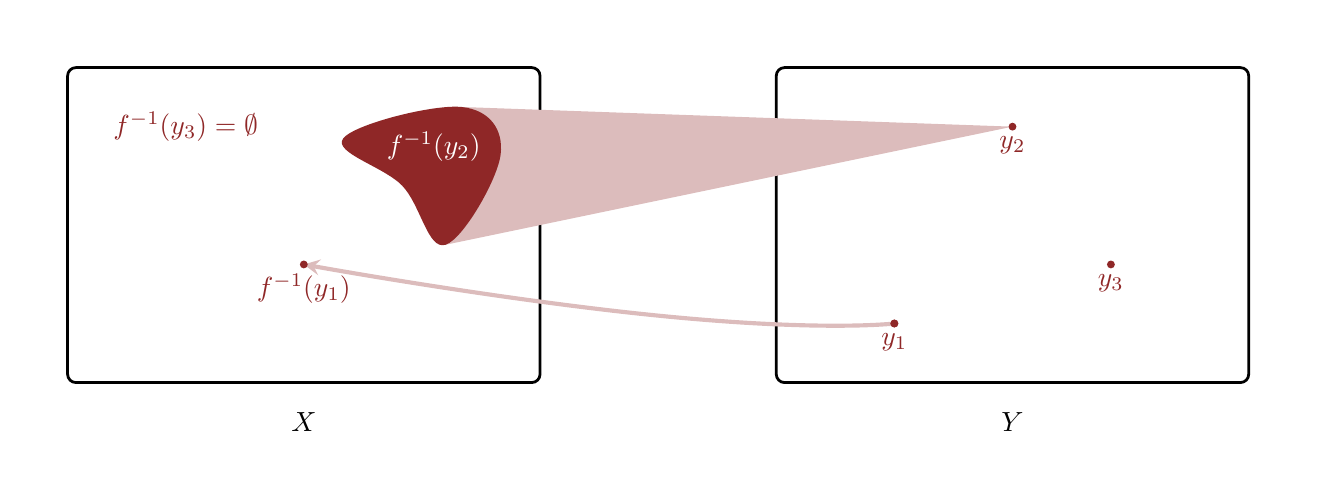
\begin{tikzpicture}[scale=1.0]
  
  \draw[white] (-3.5, -3) rectangle (12.5, 2.5);

  \begin{scope}[shift=({0, 0})]
    \draw[rounded corners=3, color=black, line width=1] (-3, -2) rectangle (3, 2);
    \node at (0, -2.5) { $X$ };
  \end{scope}

  \begin{scope}[shift=({9, 0})]
    \draw[rounded corners=3, color=black, line width=1] (-3, -2) rectangle (3, 2);
    \node at (0, -2.5) { $Y$ };
  \end{scope}
  
  \draw[light, ->, >=stealth, line width=1.5] 
    plot [smooth, tension=1] coordinates { (9 - 1.5, -1.25) (4.5, -1.15) (0, -0.5) };
  \fill[dark] (9 - 1.5, -1.25) circle (0.05);

  \fill[light] (2, 1.5) -- (9 + 0, 1.25) -- (1.8, -0.25)  -- cycle;

  \begin{scope}[shift=({0, 0})]
    \fill[dark] (0, -0.5) circle (0.05) node[below] { $f^{-1}(y_1)$ };
    
    \fill[dark] plot [smooth cycle, tension=0.65] coordinates { 
      (0.5, 1.1) (2, 1.5) (2.5, 0.9) (1.8, -0.25) (1.25, 0.5) } -- cycle;
    \node[white] at (1.65, 1) { $f^{-1}(y_2)$ };
    
    \node[dark] at (-1.5, 1.25) { $f^{-1}(y_3) = \emptyset$ };
  \end{scope}

  \begin{scope}[shift=({9, 0})]
    \fill[dark] (-1.5, -1.25) circle (0.05) node[below] { $y_1$ };
    \fill[dark] (0, +1.25) circle (0.05) node[below] { $y_2$ };
    \fill[dark] (1.25, -0.5) circle (0.05) node[below] { $y_3$ };
  \end{scope}
  
\end{tikzpicture}

\end{document}  